\chapter{Supporting materials for flexible diffusion modelling of long videos} \label{app:fdm}

\section{Experimental details}
\begin{table*}[t]
  \tiny
  \caption{Experimental details for all results reported in \cref{ch:fdm}. The GPUs referenced are all either NVIDIA RTX A5000s or NVIDIA A100s. In rows where GPU-hours are given as a range, different runs with identical settings took varying times due to varying performance of our computational infrastructure.}
  \label{tab:fdm-experimental-details}
  \centering
  \begin{tabular}{p{1.1cm}llp{0.9cm}p{0.6cm}lp{1cm}}
    \toprule
     Experiment  & Method & Res.  & Params (millions)  & Batch size  &  GPUs  & Iterations (thousands)\\
    \midrule
    \multirow{4}{*}{GQN-Mazes}         &  FDM                       & 64    & 78    & 8     & 1x A100   & 950       \\
                                       &  VDM (frameskip-1/4)       & 64    & 78/78 & 8/8   & 1x A100   & 1600/1100  \\
                                       &  TATS (VQGAN/Tran.)       & 64    & 61/423     & 96/16 & 8/8x A100 & 72/1320    \\
                                       &  CWVAE                     & 64    & 34    & 50    & 1x A100   & 110    \\
   \midrule
    \multirow{4}{*}{MineRL}            &  FDM                       & 64    & 78    & 8     & 1x A100   & 850       \\
                                       &  VDM (frameskip-1/4)       & 64    & 78/78 & 8/8   & 1x A100   & 1600/1100   \\
                                       &  TATS (VQGAN/Tran.)       & 64    & 61/423     & 96/16 & 8/8x A100   & 72/550    \\
                                       &  CWVAE                     & 64    & 34    & 50    & 1x A100   & ~60   \\
    \midrule
    \multirowcell{4}[0pt][l]{CARLA\\Town01}
                                       &  FDM                       & 128   & 80    & 8     & 4x A100   & 500       \\
                                       &  VDM (frameskip-1/4)       & 128   & 80/80 & 4/4   & 2/4x A100 & 1750/1000  \\
                                       &  TATS (VQGAN/Tran.)       & 128    & 61/423    & 48/8   & 4/4x A100   & 156/270    \\
                                       &  CWVAE                     & 64    & 34    & 50    & 1x A100   & 70      \\
   \midrule
    Ablations on GQN-Mazes   &  FDM (incl. ablations)     & 64    & 78    & 3     & 1x A5000  & 500   \\
   \midrule
    Ablations on MineRL  &  FDM (incl. ablations)     & 64    & 78    & 3     & 1x A5000  & 500       \\
    \bottomrule
  \end{tabular}
  \begin{tabular}{p{1.1cm}lllp{0.7cm}}
    \toprule
     Experiment  & Method  &  GPU-hours &  K  & Diffusion steps   \\
    \midrule
    \multirow{4}{*}{GQN-Mazes}         &  FDM                       & 156      & 20    & 1000      \\
                                       &  VDM (frameskip-1/4)       & 151/153 (total 304)   & N/A  & 1000      \\
                                       &  TATS (VQGAN/Tran.)       & 1314/1344 (total 2658)    & N/A  & N/A      \\
                                       &  CWVAE                     & 148   & N/A   & N/A       \\
   \midrule
    \multirow{4}{*}{MineRL}            &  FDM                       & 156      & 20    & 1000      \\
                                       &  VDM (frameskip-1/4)       & 161/163 (total 324)   & N/A  & 1000      \\
                                       &  TATS (VQGAN/Tran.)       & 1328/1056 (total 2384)     & N/A  & N/A      \\
                                       &  CWVAE                     & 41    & N/A    & N/A      \\
    \midrule
    \multirowcell{4}[0pt][l]{CARLA\\Town01}
                                       &  FDM                       & 380   & 20    & 1000      \\
                                       &  VDM (frameskip-1/4)       & 332/380 (total 712)   & N/A  & 1000      \\
                                       &  TATS (VQGAN/Tran.)       & 652/242 (total 894)     & N/A  & N/A      \\
                                       &  CWVAE                     & 115   & N/A   & N/A      \\
   \midrule
    Ablations on GQN-Mazes   &  FDM (incl. ablations)     & 40-70  & 10    & 250      \\
   \midrule
    Ablations on MineRL  &  FDM (incl. ablations)     & 40-70  & 10    & 250      \\
    \bottomrule
  \end{tabular}
\end{table*}

\begin{table*}[t]
  \tiny
  \caption{Additional evaluation metrics for our video completion comparisons. Lower is better for the test ``Loss'' and LPIPS. Higher is better for SSIM and PSNR.}
  \label{tab:fdm-extra-metrics}
  \centering
  \begin{tabular}{lllllllllll}
    \toprule
    \multicolumn{1}{r}{} & & \multicolumn{4}{c}{GQN-Mazes}  & \multicolumn{4}{c}{MineRL} \\
    \cmidrule(r){3-6} \cmidrule(r){7-10}
    Model &  Sampling scheme    & Loss  & LPIPS  & SSIM   & PSNR  & Loss  & LPIPS   & SSIM   &  PSNR \\
    \midrule
    \multirow{1}{*}{CWVAE~\citep{saxena2021clockwork}}& CWVAE
    & $-   $ & $0.41$  & $\textbf{0.64}$  & $16.3$  & $-   $  & $0.50$  & $\mathbf{0.59}$  & $\mathbf{19.3}$ \\
    \midrule
    \multirow{1}{*}{TATS~\citep{ge2022long}}& TATS
    & $-$ & $0.40$  & $0.59$  & $15.5$  & $-$  & $0.42$  & $0.45$  & $17.0$  \\
    \midrule
    \multirow{1}{*}{VDM~\citep{ho2022video}}& VDM
    & $\mathbf{6.04}$ & $0.39$  & $0.61$  & $16.1$  & $\mathbf{8.48}$  & $0.33$  & $0.54$  & $19.2$  \\
    \midrule
\multirow{5}{*}{FDM (ours)}   &  Autoreg
    & $6.41$ & $0.40$  & $0.60$  & $15.5$  & $9.80$  & $\mathbf{0.32}$  & $0.53$  & $18.9$  \\
                            &  Long-range
    & $6.41$ & $\mathbf{0.37}$  & $0.61$  & $16.3$  & $9.79$  & $\mathbf{0.32}$  & $0.54$  & $19.0$        \\
                            &  Hierarchy-2
    & $6.40$ & $\mathbf{0.37}$  & $0.61$  & $\mathbf{16.4}$  & $9.75$  & $0.33$  & $0.54$  & $19.0$ \\
                            &  Hierarchy-3
    & $6.38$ & $0.38$  & $0.62$  & $\mathbf{16.4}$  & $9.54$  & $0.33$  & $0.54$  & $19.1$  \\
                            &  Ad. hierarchy-2
    & $6.40$ & $\mathbf{0.37}$  & $0.62$  & $\mathbf{16.4}$  & $9.80$  & $0.33$  & $0.53$  & $19.0$ \\
    \bottomrule
  \end{tabular}
  \begin{tabular}{llllll}
    \toprule
    \multicolumn{1}{r}{} & & \multicolumn{3}{c}{CARLA Town01} \\
    \cmidrule(r){3-5}
    Model &  Sampling scheme    & LPIPS     & SSIM  & PSNR \\
    \midrule
    \multirow{1}{*}{CWVAE~\citep{saxena2021clockwork}}& CWVAE
    & $0.53$  & $0.71$  & $15.5$        \\
    \midrule
    \multirow{1}{*}{TATS~\citep{ge2022long}}& TATS
    & $0.40$  & $0.68$  & $13.9$        \\
    \midrule
    \multirow{1}{*}{VDM~\citep{ho2022video}}& VDM
    & $0.35$  & $0.71$  & $15.4$        \\
    \midrule
\multirow{5}{*}{FDM (ours)}   &  Autoreg
    & $0.28$  & $0.74$  & $17.5$        \\
                            &  Long-range
    & $\mathbf{0.26}$  & $\mathbf{0.75}$  & $\mathbf{18.5}$        \\
                            &  Hierarchy-2
    & $0.29$  & $0.73$  & $17.2$        \\
                            &  Hierarchy-3
    & $0.31$  & $0.72$  & $16.9$        \\
                            &  Ad. hierarchy-2
    & $0.30$  & $0.72$  & $17.0$        \\
    \bottomrule
  \end{tabular}
\end{table*}


The total compute required for this chapter, including all training, evaluation, and preliminary runs, was roughly 3.5 GPU-years. We used a mixture of NVIDIA RTX A5000s (on a university cluster) and NVIDIA A100s (from a cloud provider).

Due to the expensive nature of drawing samples from both FDM and our baselines, we compute all quantitative metrics reported over the first 100 videos of the test set for GQN-Mazes and MineRL. For CARLA Town01, the test set length is 100. \Cref{tab:fdm-experimental-details} lists the hyperparameters for all training runs reported. We provide additional details on the implementations of each method below.

\paragraph{FDM} 
Our implementation of FDM builds on the DDPM implementation\footnote{\url{https://github.com/openai/improved-diffusion}} of \citet{nichol2021improved}. For experiments at $64\times64$ resolution, the hyperparameters of our architecture are almost identical to that of their $64\times64$ image generation experiments: for example we use 128 as the base number of channels, the same channel multpliers at each resolution, and 4-headed attention. The exception is that we decrease the number of ResNet blocks from 2 to 1 at each up/down-sampling step. As mentioned in the main text, we run all layers from the image DDPM independently and in parallel for each frame, and add a temporal attention layer after every spatial attention layer. The temporal attention layer has the same hyperparameters as the spatial attention layer (e.g. 4 attention heads) except for the addition of relative position encodings, which we describe later. For experiments at $128\times128$ resolution, we use almost the same architecture, but with an extra block at $128\times128$ resolution with channel multiplier 1.  For full transparency, all source code is available.\footnote{\url{https://github.com/plai-group/flexible-video-diffusion-modeling}}.

\paragraph{VDM}
As mentioned in the main paper, we train VDM by simply training two networks, each with architecture identical to that of FDM but different training tasks. In each of VDM's training tasks, we use a slice of 16 or 9 frames (with frameskip 4 or 1 respectively). We randomly sample zero or more ``groups'' of regularly-spaced frames to observe (where groups of frames are sampled similarly here to in FDM's structured mask distribution in \cref{alg:mask-distribution}), and the rest are latent. On all datasets, we train each of the two networks forming the VDM baseline with roughly as many GPU-hours as FDM, so that VDM receives roughly twice as much training compute in total.

\paragraph{TATS}
We train TATS using the official implementation\footnote{\url{https://github.com/SongweiGe/TATS}} along with its suggested hyperparameters. For GQN-Mazes and MineRL we train each stage for close to a week and, following \citet{ge2022long}, train them on 8 GPUs in parallel. For all datasets, the total training computation is multiple times that of FDM. In the included video samples from our TATS baseline, some artifacts are clearly visible. It may be that these could be removed with further hyperparameter tuning, but we did not pursue this. Notably, the datasets which we experiment on generally have a lower frame-rate than those used by \citet{ge2022long}, meaning that neighboring frames are more different and so potentially harder to model.

\paragraph{CWVAE}
We train CWVAE using the official implementation\footnote{\url{https://github.com/vaibhavsaxena11/cwvae}} and use hyperparameters as close as possible to those used in the implementation by \citet{saxena2021clockwork}. We use 600 epochs to train CWVAE on MineRL, as suggested by \citet{saxena2021clockwork}, and train it for more iterations on both other datasets. On CARLA Town01, since CWVAE is not implemented for $128\times128$ images, we downsample all train and test data to $64\times64$.

\subsection{Additional evaluation metrics}
We report additional evaluation metrics in \cref{tab:fdm-extra-metrics}. 

The ``Loss'' refers to the average diffusion loss for each sampling scheme on the test set given latent and observed indices $(\gX, \gY)$ sampled according to the sampling scheme. That is, we modify the flexible diffusion loss from \cref{eq:fdm-loss} to
\begin{align} \label{eq:fdm-eval-loss}
    \mathcal{L}_\text{eval}(\theta) &= \EX_{q(\rvx, \rvx_\sigma, \rvy|\gX, \gY)u(\gX, \gY)u(\sigma)} \left[ \frac{\lambda^\rvx(\sigma)}{u(\sigma)} 
    \left\| \rvx_\theta(\rvx_\sigma, \rvy, \sigma, \gX, \gY) - \rvx \right\|_2^2 \right]
\end{align}
where $u(\gX, \gY)$ samples the index of a stage of the sampling scheme from a uniform distribution and then return the indices $\gX$ and $\gY$ used at that stage of the sampling scheme. An appropriate choice of $\lambda(\sigma)$ would lead \cref{eq:fdm-eval-loss} to lower-bound the likelihood of generating our test set given our model and sampling scheme but, as in our training loss, we instead use the ``uniform-weighting'' proposed by \citet{ho2020denoising}. This de-emphasises pixel-level detail. 

The commonly-used~\citep{saxena2021clockwork,babaeizadeh2021fitvid} LPIPS, SSIM and PSNR metrics measure frame-wise distances between each generated frame around the ground-truth. To account for stochasticity in the task, $k$ video completions are generated for each test video and the smallest distance to the ground-truth is reported. We report them for completeness, but do not believe that SSIM and PSNR correlate well with video quality due to the stochastic nature of our datasets. For example, we report MineRL videos sampled with CWVAE\footnote{\url{https://www.cs.ubc.ca/~wsgh/fdm}} which obtain higher (better) SSIM and PSNR than other methods despite being much blurrier. Since SSIM and PSNR are related to the mean-squared error in pixel space, they favour blurry samples over more realistic samples. While increasing $k$ should counteract this effect, the effectiveness of doing so decreases with video length and and so increasing $k$ made little difference in the datasets we consider.


\section{Explanation of our training task distribution} \label{app:training-task-dist-exp}
Here we provide our motivation, design choices and more explanation of our training task distribution, as visualized in \cref{fig:training-distribution} and implemented in \cref{alg:training-distribution}. Since we train our model to work with any custom sampling scheme at test time, our training distribution should be broad enough to assign some probability to any feasible choices of frames to sample and observe. At the same time, we want to avoid purely random sampling of frame positions (as in e.g. the ablation in \cref{ap:fdm-training-task-distribution-ablation}) as this will impair performance in realistic sampling schemes. Taking these considerations in mind, our design considerations for \cref{alg:training-distribution} are simple:
\begin{enumerate}
    \item The model should sample frames at multiple timescales, so we sample the spacing between frames (as on line 4 of \cref{alg:training-distribution}). A log-uniform distribution is a natural fit since events in a video sequence can happen over timescales in, e.g., seconds, minutes, or hours, and the differences between these are best captured by a log scale. The parameters of this log-uniform distribution are chosen to be the broadest possible (given the video length and the frame rate).
    \item The user may wish to jointly sample multiple disparate sections of a video. We therefore make it possible to sample multiple groups of frames, potentially with different timescales (this is the purpose of the while loop in \cref{alg:training-distribution}).
    \item The number of frames a user may wish to sample at a time is not fixed, so we add a broad uniform distribution over this (line 3 of the algorithm).
    \item We train the model to perform conditional generation, so we choose groups of frames to be conditioned on (line 6 of the algorithm) using the simplest appropriate distribution, Bernoulli(0.5).
\end{enumerate}
The remainder of the algorithm is boilerplate, gathering the indexed frames (line 1, 7, 9-13), randomising the position of frames within the video (line 5) and enforcing that the number of frames does not exceed $K$ (line 8). Note that we do not claim that e.g. this exact mechanism for ensuring that $\leq K$ frames are sampled is a necessary or optimal choice for achieving FDM’s performance. It is simply a design choice.

\subsection{Ablation on training task distribution} \label{ap:fdm-training-task-distribution-ablation}
We mention in the main paper that we perform an ablation on the training task distribution. FVD scores from this ablation are reported in \cref{tab:fdm-task-dist-ablation}. We sample from the baseline ``uniform'' task distribution as follows (where $\text{Uniform(a, b)}$ should be understood to assign probability to all integers between $a$ and $b$ \textit{inclusive}):
\begin{enumerate}
    \item Sample $n_{total} \sim \text{Uniform}(1, K)$.
    \item Assign $\mathcal{Z}$ to be a vector of $n_{total}$ integers sampled without replacement from $\{1,\ldots,N\}$.
    \item Sample $n_{obs} \sim \text{Uniform}(0, n_{total}-1)$.
    \item Assign the first $n_{obs}$ entries in $\mathcal{Z}$ to $\obsindices$ and the remainder to $\latindices$.
\end{enumerate}
This leads to a much less structured distribution than that described in \cref{fig:training-distribution}. The network trained using our proposed task distribution obtains a better FVD than our ablation on all tested combinations of dataset and sampling scheme. Note that all networks in this experiment use the hyperparameters reported in the bottom two rows of \cref{tab:fdm-experimental-details}, explaining the disparity between FVDs here and in \cref{tab:fdm-results-completion}.
\begin{table}[t]
    \centering
    \small
    \caption{Ablation on our flexible video diffusion model's training task distribution.}
    \label{tab:fdm-task-dist-ablation}
    \begin{tabular}{l|l|ll}
    \toprule
        ~ & ~ & FDM & Uniform \\%& w/ 1 group \\ 
        \midrule
        \multirow{5}{*}{GQN-Mazes} & Autoreg & \textbf{245} & 327 \\%& 260 \\ 
        ~ & Hierarchy-2 & \textbf{235} & 279 \\%& 202 \\ 
        ~ & Long-range & \textbf{198} & 281 \\%& 238 \\ 
        ~ & Hierarchy-3 & \textbf{176} & 284 \\%181 \\
        ~ & Ad. hierarchy-2 & \textbf{178} & 281 \\%184 \\
        ~ & Average & \textbf{226} & 296 \\%233 \\  
        \midrule
        ~ & Autoreg & \textbf{465} & 672 \\%~ \\ 
        ~ & Hierarchy-2 & \textbf{586} & 902 \\%~ \\ 
        MineRL & Long-range & \textbf{504} & 783 \\%~ \\ 
        ~ & Hierarchy-3 & \textbf{515} & 970 \\%~ \\ 
        ~ & Ad. hierarchy-2 & \textbf{613} & 990 \\%~ \\ 
        ~ & Average & \textbf{518} & 786 \\%~ \\ 
        \bottomrule
    \end{tabular}
\end{table}


\section{Relative position encodings} \label{app:fdm-rpe}


\paragraph{Relative position encoding background and use-case} Our temporal attention layer is run independently at every spatial location, allowing each spatial location in every frame to attend to its counterparts at the same spatial location in every other frame. That is, denoting the input to a temporal attention layer $\rvz^\text{in}$ and the output $\rvz^\text{out}$, we compute the $K \times C$ slice $\rvz^\text{out}_{:,h,w,:} = \text{attn}(\rvz^\text{in}_{:,h,w,:})$ for every spatial position $(h,w)$. To condition the temporal attention on the frame's positions within the video, we use relative position encodings (RPEs)~\citep{shaw2018self,wu2021rethinking} for each pair of frames. Let $pos(i) = (\latindices\oplus\obsindices)_i$ be a function mapping the index of a frame within $\rvz$ to its index within the full video $\rvv$. Then the encoding of the relative position of frames $i$ and $j$ depends only on $pos(i)-pos(j)$. We write this RPE as the set of three vectors $\rp_{ij} = \{\rp_{ij}^Q, \rp_{ij}^K, \rp_{ij}^V\}$ which are used in a modified form of dot-product attention (described in the following paragraph). Since $\rp_{ij}$ must be created for every $(i,j)$ pair in a sequence, computing it adds a cost which scales as $\mathcal{O}(K^2)$ and prior work has attempted to minimise this cost by parameterising $\rp_{ij}$ with a simple learned look-up table (LUT) as ${\rp_{ij} := \text{LUT}(pos(i)-pos(j))}$. In the next paragraph we describe our alternative to the LUT, but first we describe how the RPEs are used in either case. We use the RPEs in the same way as \citet{shaw2018self}. As in a standard transformer~\citep{vaswani2017attention}, a sequence of input vectors $\rvz_1^\text{in},\ldots,\rvz_{K}^\text{in}$ are transformed to queries, keys, and values via the linear projections $\rvq_i = W^Q \rvz_i$, $\rvk_i = W^K \rvz_i$, and $\rvv_i = W^V \rvz_i$ for $i=1,\ldots,K$. Given the RPEs for all $(i,j)$ pairs, and marking the operations involving them in \textcolor{blue}{blue}, the output of the attention block is
\begin{align}
    \rvz_i^\text{out} = \rvz^\text{in}_i + \sum_{j=1}^K \alpha_{ij}(\rvv_j \textcolor{blue}{+ \rp_{ij}^V}) \quad \text{where} \quad \alpha_{ij} &= \frac{\exp(e_{ij})}{\sum_{k=1}^K\exp(e_{ik})} \\
    \text{with} \quad e_{ij} &= \frac{1}{\sqrt{d_z}} \left( \rvq_i^\intercal \rvk_j \textcolor{blue}{+ {\rp_{ij}^Q}^\intercal \rvk_j + \rvq_i^\intercal {\rp_{ij}^K}} \right). \nonumber
\end{align}

\begin{figure}[t]
  \begin{center}
    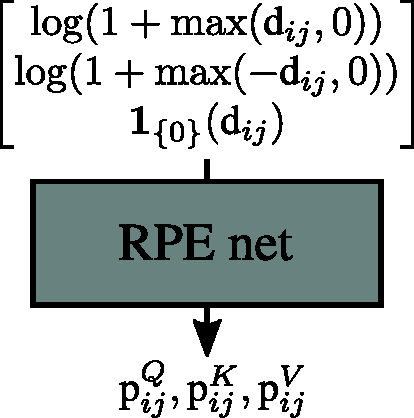
\includegraphics[width=0.3\textwidth]{figs/fdm/rpe-net.pdf}
  \end{center}
  \caption{Architecture diagram for $f_\text{RPE}$, the neural network which produces relative position embeddings given input $\rd_{ij} := pos(i)-pos(j)$.}
  \label{fig:fdm-rpe-net}
\end{figure}

\paragraph{Our approach to computing RPEs}
We argue that the simplicity of parameterising RPEs with a LUT is not necessary within our framework for three reasons. 
\textbf{(1)} In our framework, $K$ can be kept small, so the $\mathcal{O}(K^2)$ scaling cost is of limited concern. 
\textbf{(2)} Furthermore, since the temporal attention mechanism is run for all spatial locations $(h, w)$ in parallel, the cost of computing RPEs can be shared between them.
\textbf{(3)} The range of values that $pos(i)-pos(j)$ can take scales with the video length $N$, and the average number of times that each value is seen during training scales as ${K^2/N}$. For long videos and small $K$, a look-up table will be both parameter-intensive and receive a sparse learning signal. 
%
We propose to parameterise $\rp_{ij}$ with a learned function as ${\rp_{ij} := f_\text{RPE}(\rd_{ij})}$ where $\rd_{ij} := pos(i)-pos(j)$. As shown in \cref{fig:fdm-rpe-net}, $f_\text{RPE}$ passes a 3-dimensional embedding of $\rd_{ij}$ through a neural network which outputs the vectors making up $\rp_{ij}$. We use a network with a single $C$-channel hidden layer and were not able to measure any difference in the runtime between a DDPM with this network and a DDPM with a look-up table.  \Cref{fig:fdm-rpe-net-attn-weights} shows the effect of the RPE network on attention weights early in training. Architectures with an RPE network can learn the relative importance of other frames much more quickly. After training to convergence, there was no noticeable difference in sample quality but the architecture with an RPE network used 9.8 million fewer parameters by avoiding storing large look-up tables.

An alternative approach to our RPE network described by \citet{wu2021rethinking} shares the look-up table entries among ``buckets'' of similar $pos(i)-pos(j)$, but this imposes additional hyperparameters as well as restricting network expressivity.

\begin{figure}
    \centering
    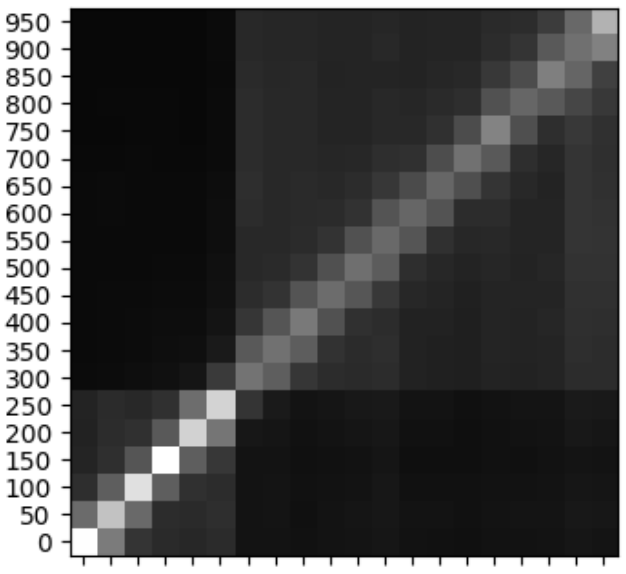
\includegraphics[width=0.25\textwidth]{figs/fdm/attn_masks/w_rpe.png}
    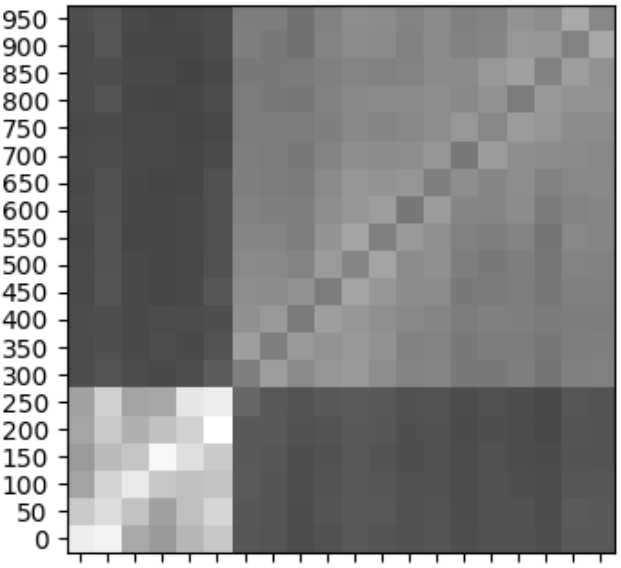
\includegraphics[width=0.25\textwidth]{figs/fdm/attn_masks/wo_rpe.png}
    \caption{Visualisation of temporal attention weights. The weights displayed are averaged over attention heads, spatial locations, network layers, and diffusion timesteps 1000 to 751. The colour of entry $r,c$ is proportional to the average weight with which the $r$th frame in $\rvx\oplus\rvy$ attends to the $c$th frame. Black means zero weight. We plot an example where $\obsindices=\{0,50,\ldots,250\}$ and $\latindices=\{300, 350,\ldots,950\}$. These plots are made with a network trained for 50\,000 iterations of training on the CARLA Town01 dataset. \textbf{Left:} From an architecture with an RPE network. \textbf{Right:} From a network with look-up tables of relative position embeddings. The architecture with an RPE network in the left plot has already learned to assign much greater weight to the nearest frames, while e.g. latent frames attend almost uniformly to other latent frames in the right plot. After training to convergence, both plots look similar to that on the left.  }
    \label{fig:fdm-rpe-net-attn-weights}
\end{figure}



\section{Sampling schemes}
\Cref{fig:fdm-sampling-schemes} illustrates each of the sampling schemes for which we reported results. We show the versions adapted to completing 300-frame GQN-Mazes videos from 36 initial observations, but all can be extended to e.g. different video lengths.
\begin{figure}[t]
    \centering
    \begin{subfigure}[t]{\textwidth}
        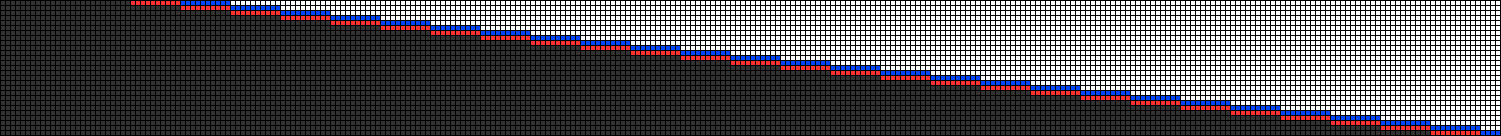
\includegraphics[width=\textwidth]{figs/fdm/inference-modes/sample_vis_autoreg_T=300_sampling_10_out_of_20_red_blue_flipped.png}
        \caption{Autoreg.}
    \end{subfigure}
    \begin{subfigure}[t]{\textwidth}
        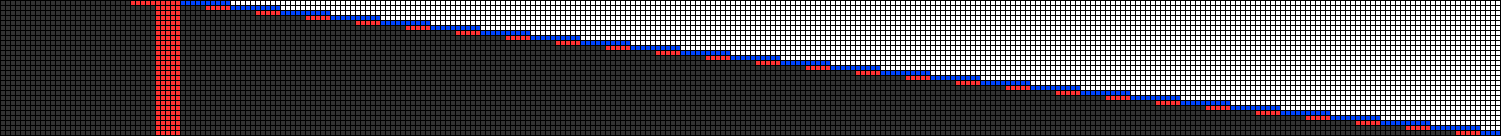
\includegraphics[width=\textwidth]{figs/fdm/inference-modes/sample_vis_mixed-autoreg-independent_T=300_sampling_10_out_of_20_red_blue_flipped.png}
        \caption{Long-range.}
    \end{subfigure}
    \begin{subfigure}[t]{\textwidth}
        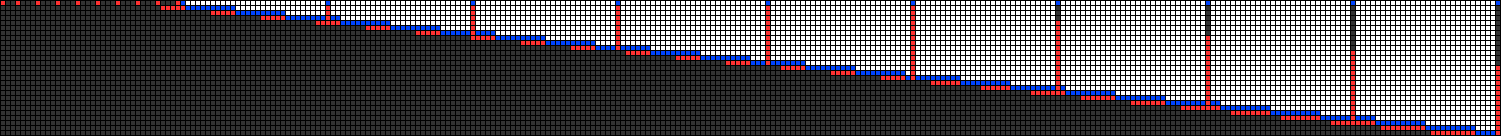
\includegraphics[width=\textwidth]{figs/fdm/inference-modes/sample_vis_hierarchy-2_T=300_sampling_10_out_of_20_red_blue_flipped.png}
        \caption{Hierarchy-2.}
    \end{subfigure}
    \begin{subfigure}[t]{\textwidth}
        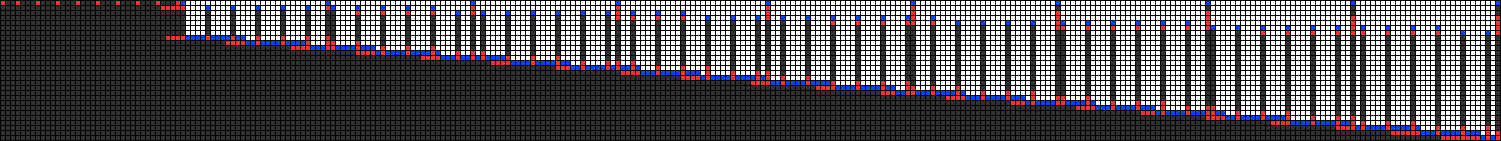
\includegraphics[width=\textwidth]{figs/fdm/inference-modes/sample_vis_hierarchy-3_T=300_sampling_10_out_of_20_red_blue_flipped.png}
        \caption{Hierarchy-3.}
    \end{subfigure}
    \begin{subfigure}[t]{\textwidth}
        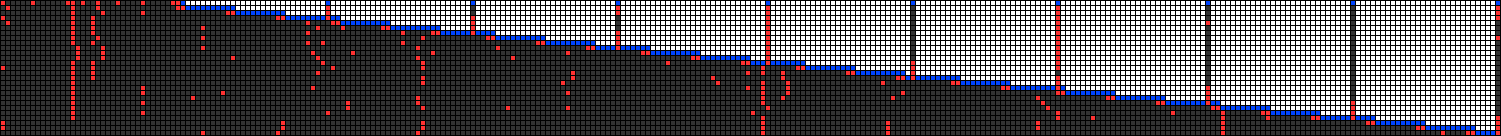
\includegraphics[width=\textwidth]{figs/fdm/inference-modes/sample_vis_adaptive-hierarchy-2_T=300_sampling_10_out_of_20_index-0_red_blue_flipped.png}
        \caption{Ad. hierarchy-2. Frame indices shown for one particular test video.}
    \end{subfigure}
    \begin{subfigure}[t]{\textwidth}
        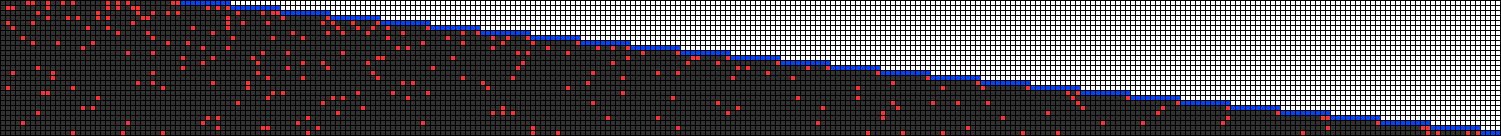
\includegraphics[width=\textwidth]{figs/fdm/inference-modes/sample_vis_autoreg_optimal-linspace-t-force-nearby_T=300_sampling_10_out_of_20_red_blue_flipped.png}
        \caption{Opt. autoreg. Observed indices are optimized for the GQN-Mazes dataset.} \label{fig:fdm-opt-autoreg}
    \end{subfigure}
    \begin{subfigure}[t]{\textwidth}
        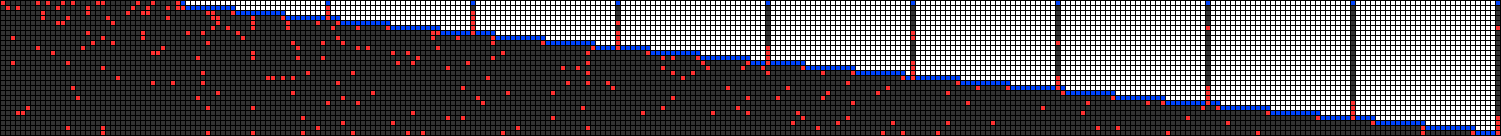
\includegraphics[width=\textwidth]{figs/fdm/inference-modes/sample_vis_hierarchy-2_optimal-linspace-t-force-nearby_T=300_sampling_10_out_of_20_red_blue_flipped.png}
        \caption{Opt. hierarchy-2. Observed indices are optimized for the GQN-Mazes dataset.} \label{fig:fdm-opt-hierarchy-2}
    \end{subfigure}
    \begin{subfigure}[t]{\textwidth}
        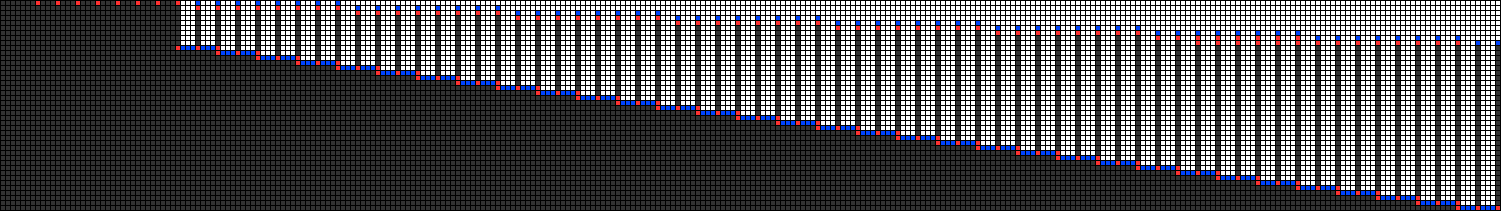
\includegraphics[width=\textwidth]{figs/fdm/inference-modes/sample_vis_google_T=300_sampling_None_out_of_None_red_blue_flipped.png}
        \caption{VDM. Like \citet{ho2022video}, we use two DDPMs to sample from this scheme.}
    \end{subfigure}
    \caption{Visualisations of all sampling schemes used in our experiments on the GQN-Mazes dataset.}
    \label{fig:fdm-sampling-schemes}
\end{figure}


\subsection{Adaptive sampling schemes} \label{ap:fdm-adaptive}
As mentioned in the main text, our Ad. hierarchy-2 sampling scheme chooses which frames to condition on at test-time by selecting a diverse set of observed of previously generated frames. Our procedure to generate this set is as follows. For a given stage $s$ we define $\latindices_s$ to be the same as the latent frame indices at the corresponding stage of the standard Hierarchy-2 sampling scheme. We then initialise $\obsindices_s$ with the closest observed or previously generated frame before the first index in $\latindices_s$, after the last index in $\latindices_s$, and any observed or previously generated frames between the first and last indices of $\latindices_s$. We add more observed indices to $\obsindices_s$ in an iterative procedure, greedily adding the observed or previously generated frame with the maximum LPIPS~\cite{zhang2018unreasonable} distance to it's nearest neighbour in $\obsindices_s$. Frames are added one-at-a-time in this way until $\obsindices_s$ is the desired length (generally $K/2$, or 10 in our experiments). Despite using a convolutional neural network to compute the LPIPS distances, the computational cost of computing $\obsindices_s$ in our experiments with Ad. hierarchy-2 is small relative to the cost of drawing samples from the DDPM.


\subsection{Optimised sampling schemes}
We now describe in detail our procedure for optimising the choice of indices to condition on at each stage in a sampling scheme. Our procedure requires that the ``latent'' frames are pre-specified. \Cref{fig:fdm-opt-autoreg,fig:fdm-opt-hierarchy-2} show examples of the indices that our optimisation scheme chooses to condition on for GQN-Mazes when the latent indices are set according to either our Autoreg or Hierarchy-2 sampling scheme. We emphasise that the (relatively computationally-expensive) optimisation described in this section need only be performed once and then arbitrarily many videos can be sampled. This is in contrast to the adaptive sampling scheme described in \cref{ap:fdm-adaptive}, in which the sets of indices to condition on are chosen afresh (with small computational cost) for each video as it is sampled. For each stage of the sampling scheme, we select the set of indices to condition on with a greedy sequential procedure as follows. 

\paragraph{Intialisation of $\obsindices$}
This procedure begins by initialising this set of indices, $\obsindices$. In general $\obsindices$ can be initialised as an empty set, but it can also be initialised with indices that the algorithm is ``forced'' to condition on. We initialise it to contain the closest observed/previously sampled indices before and after each latent index. In other words, we initialise it so that there is a red pixel between any blue and grey pixel in each row of \cref{fig:fdm-opt-autoreg,fig:fdm-opt-hierarchy-2}.

\paragraph{Appending to $\obsindices$}
On each iteration of the procedure, we estimate the evaluation loss (with uniform weighting) for every possible next choice of index to condition on. That is, we compute
\begin{align}
    \mathcal{L}_\text{eval}(\theta) &= \EX_{q(\rvx, \rvx_\sigma, \rvy|\gX, \gY')u(\sigma)} \left[ \frac{\lambda^\rvx(\sigma)}{u(\sigma)}
    \left\| \rvx_\theta(\rvx_\sigma, \rvy, \sigma, \gX, \gY') - \rvx \right\|_2^2 \right] \mathrm{d}\sigma
\end{align}
for the $\gX$ pre-specified at that sampling scheme stage and for $\gY' = \gY \oplus [i]$ for every possible next index ${i\in\{1,\ldots,N\}\setminus\latindices\setminus\obsindices}$.
% when conditioning on frames at indices ${\obsindices \oplus [i]}$ for every ${i\in\{1,\ldots,N\}\setminus\latindices\setminus\obsindices}$. 
Rather than doing true Monte-Carlo sampling, we approximate this expectation by only evaluating at $\sigma$ corresponding to timesteps ${t \in \{100,200,\ldots,1000\}}$ and, for each timestep, estimating the expectation over $\rvx$ with 10 different training images. We found that the iteration over a grid of timesteps, rather than random sampling, helped to reduce the variance in our loss estimates and so make them more comparable between different choices of index $i$. We finally select the index $i$ resulting in the lowest evaluation loss, append it to $\obsindices$, and repeat until $\obsindices$ is at the desired length. We repeat this entire procedure to build $\gY$ for every stage of the sampling scheme.

\section{CARLA Town01}
The CARLA Town01 dataset was created by recording a simulated car driving programatically around the CARLA simulator's Town01~\cite{dosovitskiy2017carla}. The car is driven so as to stay close to the speed limit of roughly $3$m/s where possible, stopping at traffic lights. The simulations run for 10\,000 frames and we split each into 10 1000-frame videos.\footnote{Due to technical glitches, not all simulations finished. When these occur, we simply save however many 1000-frame videos have been generated.} Within each simulation, the weather and other world state (e.g. state of the traffic lights) is sampled randomly. The car begins each simulation in a random position, and navigates to randomly selected waypoints around the town. As soon as it reaches one, another is randomly sampled so that it continues moving. We use a 120 degree field of view and render frames at $128\times128$ resolution.
%
To perform our evaluations on this dataset, we trained a regressor to map from a frame (either from the dataset or from a video model) to the corresponding town coordinates. This is trained with $(x,y)$ coordinates extracted from the simulator corresponding to the car location at each frame. The regressor takes the form of two separate networks: a classifier mapping each frame to a cell within a $10\times10$ grid placed over the town; and a multi-headed regressor mapping from the frame to $(x,y)$ coordinates in a continuous space. The final layer of the multi-headed regressor consists of 100 linear ``heads'', and which one to use for each data point is chosen depending on which cell the coordinate lies in. These two networks are trained separately but used jointly during evaluation, when the classifier is run first and its output determines which regressor head is used to obtain the final $(x,y)$ coordinate. We found that this approach improved the test mean-squared error considerably relative to using a single-headed regressor. The classifier was trained with data augmentation in the form of colour jitter and a Gaussian blur, but we found that the multi-headed regressor did not benefit from this data augmentation so trained it without. Both the classifier and multi-headed regressor had the Resnet128~\citep{he2015deep} architecture, with weights pretrained on ImageNet, available for download from the PyTorch torchvision package~\citep{paszke2017automatic}. We will release the classifier and multi-headed regressor used to evaluate our models, enabling future comparisons.

\begin{figure}
    \centering
    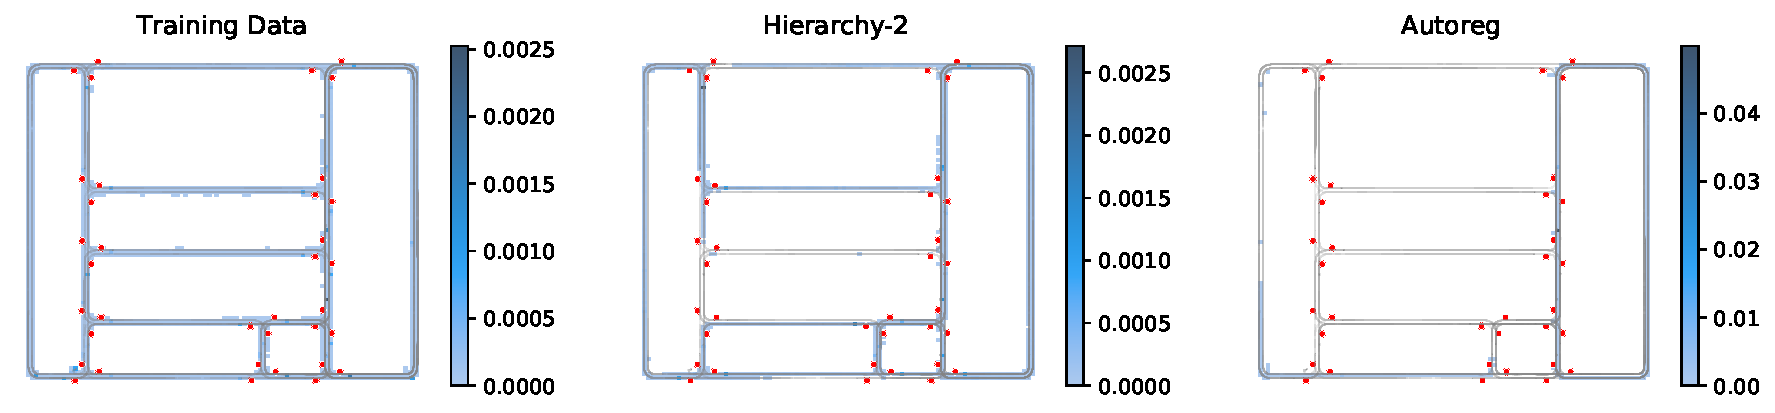
\includegraphics[width=\textwidth]{figs/fdm/heatmap.pdf}
    \caption{Heatmap of locations visited in (left) the CARLA Town01 training data, (middle) our long video sampled with Hierarchy-2, and (right) our long video sampled with Autoreg. The intensity of the blue colour corresponds to the percentage of time spent in a given location and red dots mark the locations of traffic lights. Both sampled videos stop in locations in which the vehicle also stopped in the training data (shown as darker blue spots on the heatmap), corresponding to traffic light positions. The training data contains several days of video, so covers the map well. Each sampled trajectory lasts for 30-40 minutes so should not be expected to explore the entire map. However, Hierarchy-2 in particular obtains high coverage. The video sampled with Autoreg explores less of the map due to its tendency to remain stationary for long periods.  }
    \label{fig:fdm-carla-long-video-heatmap}
\end{figure}



\section{Sampled videos}
To fully appreciate our results, we invite the reader to view a collection of FDM's samples in mp4 format.\footnote{\url{https://www.cs.ubc.ca/~wsgh/fdm}} These include video completions, unconditionally sampled videos, and the long video samples from which some frames are shown in \cref{fig:fdm-1}. To summarise the long video samples in this document, we visualise the trajectories taken throughout their (30-40 minute) course on CARLA Town01 in \cref{fig:fdm-carla-long-video-heatmap}.
Additionally, in the following pages, we show frames from uncurated samples of both video completions and unconditional video generations on each dataset.


\begin{figure}[b]
    \centering
    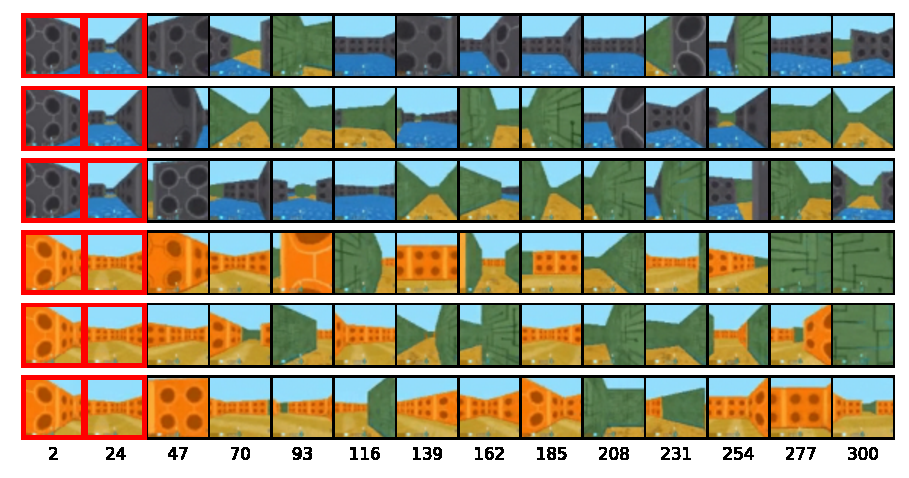
\includegraphics[width=0.8\textwidth]{figs/fdm/mazes-cond.pdf}
    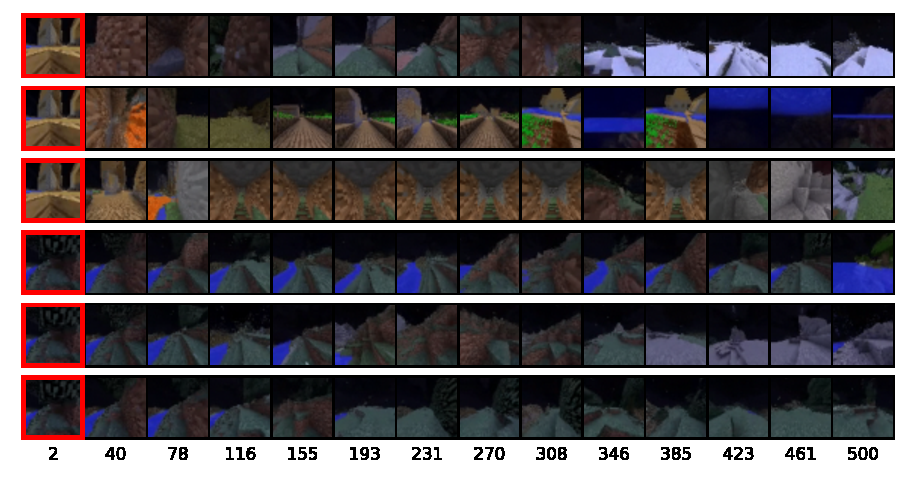
\includegraphics[width=0.8\textwidth]{figs/fdm/minerl-cond.pdf}

    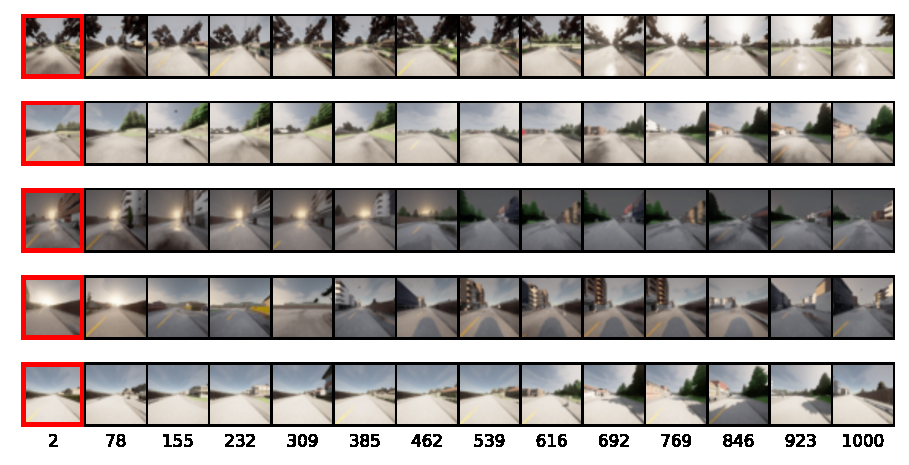
\includegraphics[width=0.8\textwidth]{figs/fdm/carla-cond.pdf}
    \caption{Video completions sampled by our method for each of GQN-Mazes, MineRL, and CARLA Town01. All are sampled with Hierarchy-2. The first 36 frames are observed, indicated by a red border. Notably, the samples on GQN-Mazes do not exhibit the failure mode seen in \cref{fig:fdm-mazes-autoreg}.}
    \label{fig:fdm-all-cond}
\end{figure}

\begin{figure}
    \centering
    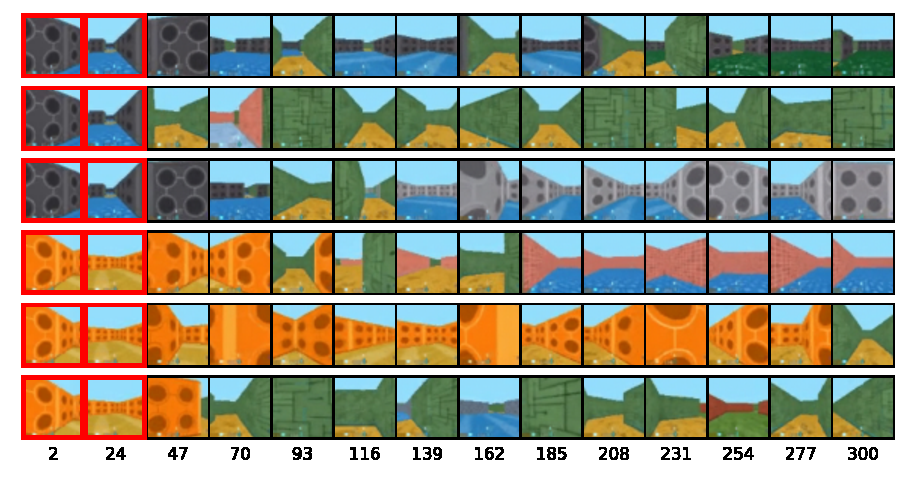
\includegraphics[width=0.8\textwidth]{figs/fdm/mazes-autoreg.pdf}
    \caption{Video completions on GQN-Mazes sampled with Autoreg. To match the data distribution there should only be two wall/floor colours within each video, but Autoreg often samples more as it cannot track long-range dependencies. This issue is not seen in the Hierarchy-2 samples shown in \cref{fig:fdm-all-cond}.}
    \label{fig:fdm-mazes-autoreg}
\end{figure}


\begin{figure}
    \centering
    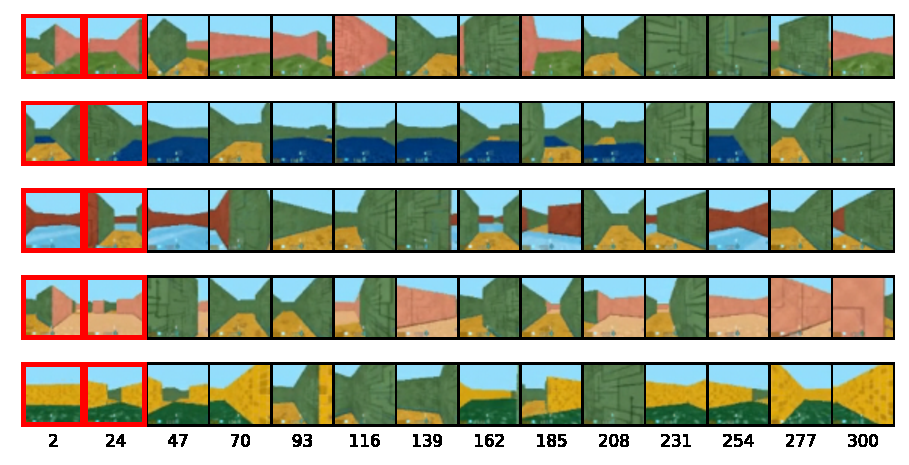
\includegraphics[width=0.8\textwidth]{figs/fdm/mazes-uncond.pdf}
    \label{fig:fdm-mazes-uncond}
    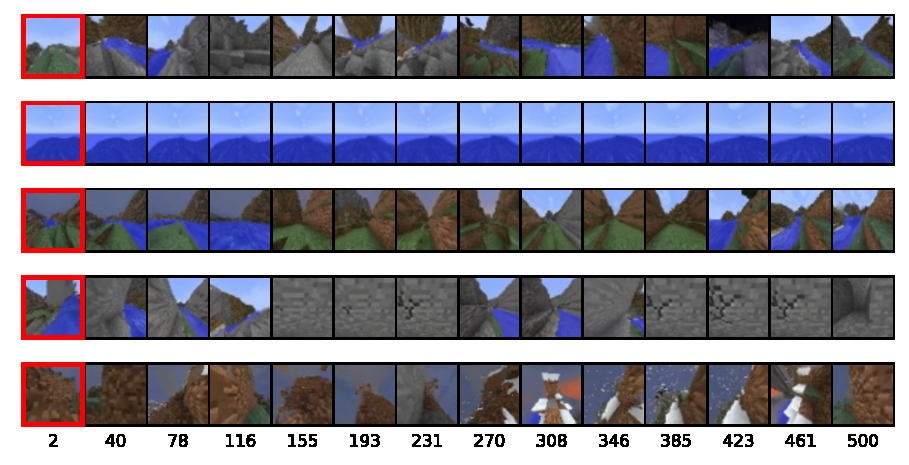
\includegraphics[width=0.8\textwidth]{figs/fdm/minerl-uncond.pdf}
    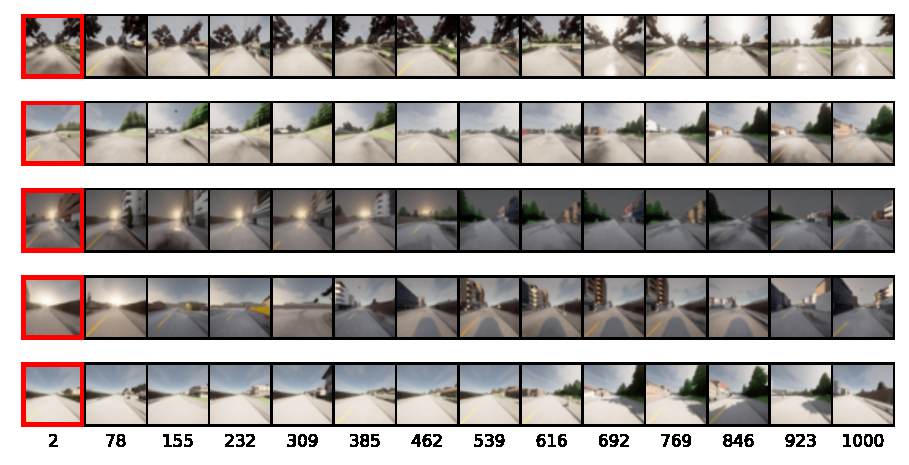
\includegraphics[width=0.8\textwidth]{figs/fdm/carla-uncond.pdf}
    \caption{Videos sampled unconditionally by FDM with Hierarchy-2 on each dataset.}
    \label{fig:fdm-carla-uncond}
\end{figure}
